\chapter{The Camera Response}
\label{chap:crf}
In the following paragraph, the essential terminology for this thesis is introduced in combination with a short overview. In \autoref{fig:crfoverview}, a visualized overview is given.

\emph{Scene radiance} is the composition of the real-world radiances in the natural scene, \hbox{i.e.} the amount of light. Note that scene radiance is only dependent on the physics of the scene. It is not yet affected by any technically induced disturbances. Then scene radiance is transformed to \emph{image irradiance} through measuring discrete intensity values on a light-sensitive sensor array, most commonly a CCD chip for digital cameras. With some special cameras designed for scientific purposes, it is now possible to extract such RAW images. But most commonly, the output of a digital camera -- after the post-processing of the image irradiance by a camera-internal processor -- is \emph{image intensity}.
In this work, the focus is on the determination of major changes between two consecutive in-camera transformations.

\begin{figure}[p]
	\centering
	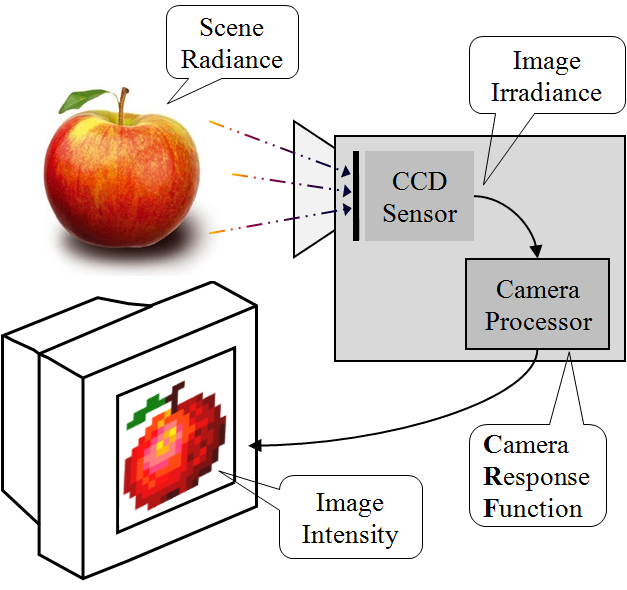
\includegraphics[width=0.8\textwidth]{images/crf_overview.png}
	\caption[On the overview terminology]{On the overview terminology. The apple in the upper left illustrates a real-world scene. The grey box on the right represents a simplified digital camera, where at first light is measured through a CCD sensor and its output is afterwards post-processed by the camera-internal processor. This is where the CRF is applied. The output of the processor -- an intensity image -- is shown in the lower left (on the computer monitor).}
	\label{fig:crfoverview}
\end{figure}

\section{Measuring Scene Radiance}
\label{sec:radiancetoirradiance}
For measuring natural scene radiance, a \emph{charge-coupled device} (CCD) sensor -- invented in 1969 -- is most commonly used in consumer-quality digital cameras. Through a lens, light is projected on a photoactive array, where in each cell electric charge proportional to the amount of incoming light (photons) at that specific location is accumulated. After this so-called exposure period, the process of transferring the charge off the array begins. For each row in the array, the charge in each cell is shifted until reaching the corner cell, where the charge is converted into voltage, measured by an analog-to-digital converter and finally transferred to memory. Once all the cells in a row have been processed, the cells in the next row get measured. Although each cell and each row is measured individually, millions of cells can be sampled in a fraction of a second.

The just described functional principle of a CCD sensor measures light, not color. For that reason, digital cameras most commonly use a \emph{Bayer mask} attached to the CCD sensor to get three channel RGB information, where each $2 \times 2$ square on the CCD array has one pixel filtered red, one pixel filtered blue and two pixels filtered green (see \autoref{fig:bayermask}). The high amount of green filtered pixels is chosen due to the fact that the human eye also is much more sensitive to green than either red or blue. The filter makes the color resolution per pixel lower, but still the luminance information is collected at every pixel. The filtering causes a \emph{mosaicing} effect on the resulting CCD output, such that the final intensity image has to be reconstructed from these color CCD samples. For this purpose, \emph{demosaicing} techniques as in \cite{kimmel1998demosaicing} are available. Although better color resolution can be reached by using so-called 3CCD devices, where for each of the three colors -- red, green and blue -- a separate CCD chip is used after the light is separated by a prism, most digital cameras have a single CCD sensor built in due to significantly lower manufacturing costs.

\begin{figure}[t]
	\centering
	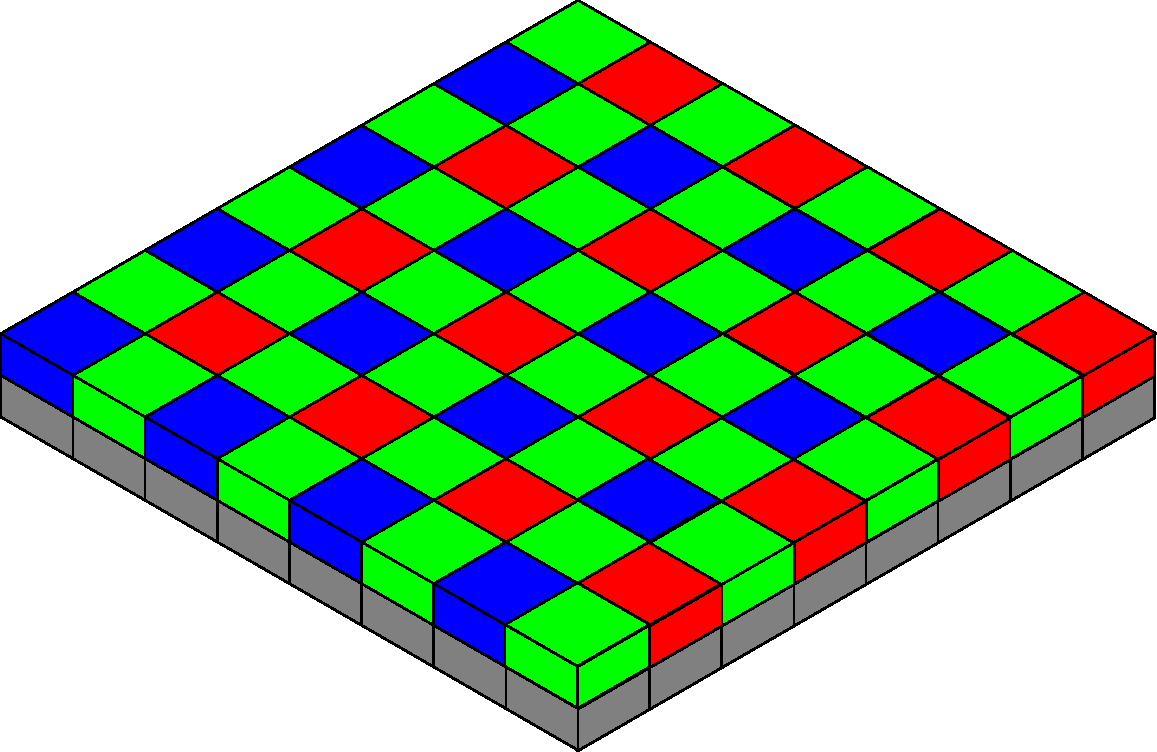
\includegraphics[width=0.5\textwidth]{images/bayerfilter.pdf}
	\caption[Bayer filter on a CCD sensor]{Bayer filter on a CCD sensor. The colored boxes sketch the Bayer mask and the underlying grey boxes the cells of the actual CCD sensor array. Note that the amount of green filtered pixels is as high as the amount of pixels for the colors red and blue combined.}
	\label{fig:bayermask}
\end{figure}

The charge in each cell is proportional to the luminance. Thus, the function, which maps scene radiance to image irradiance, is basically linear, although it may vary spatially over the image due to the presence of noise. Examining the effects caused by this transformation for going from image irradiance back to scene radiance are not part of this thesis. For further reference, confer \cite{healey1994radiometric}.


\section{Mapping Image Irradiance to Image Intensity (CRF)}
\label{sec:irradiancetointensity}
The camera response function maps image irradiance to image intensity. Having a wide range of irradiance values and just a small range of possibly measurable intensity values, nonlinearity is a simple method for compressing these values. So camera manufacturers purposefully introduce nonlinearities in the camera's electronics, \hbox{i.e.} nonlinear CRFs. A second reason is, that a few years ago, digital cameras were not yet available for the consumer market. Typically, analog cameras with photographic films were used to take photographs. So the first digital cameras aimed to mimic the properties of analog photographs, which were usually nonlinear as well. Furthermore, a variety of aesthetic effects and refinements with respect to human perception can be generated by varying the CRF, like applying gamma correction, white balancing to compensate for different light temperature or other sophisticated corrections to make the image more visually appealing.

M. Grossberg and S. Nayar examined the CRFs of 201 real-world digital cameras and video cameras as well as common brands of films. They compiled a database of real-world camera response functions (DoRF), available on their website\footnote{\url{http://www.cs.columbia.edu/CAVE/software/softlib/dorf.php}}. Their intention was to build up a solid ground-truth base for evaluating different camera response models. This database is now also used as prior knowledge for maximum a posteriori (MAP) estimations in \cite{Lin04radiometriccalibration}. All CRFs in DoRF are monotonic and normalized to $[0; 1]$.

A common assumption on CRFs is, that it is the same for each pixel in image irradiance, although in theory the CRF could vary spatially. The second assumption is that every camera response has a well defined boundary $B$, where the CRF domain goes from $B_\text{min}$ to $B_\text{max}$. Both variables can be computed easily. $B_\text{min}$ can be estimated by taking a photo with the lens cap on, $B_\text{max}$ on the other hand by photographing a very bright object such as the sun or other light sources. Parts of the image will then be saturated. Having this boundary for a camera, it is reasonable to normalize the domain to $[0; 1]$ as done in the following.
\begin{equation}
	\overline{x} = \frac{x - B_\text{min}}{B_\text{max} - B_\text{min}}, \ \ x \in B = [B_\text{min}; B_\text{max}] \enspace ,
	\label{eq:normalization}
\end{equation}
where $x$ is a measured irradiance value and $\overline{x}$ its normalization. The codomain of a CRF is also normalized, with respect to the number of available bits $\#_b$ per channel, which is usually $\#_b = 8$. So $B_\text{min} = 0$ and $B_\text{max} = 2^{\#_b}-1$ in terms of \autoref{eq:normalization}. 

The third assumption is that any CRF $f$ is strictly monotonically increasing, what makes the CRF invertible. Hence, once the CRF is determined, it can get inverted to map image intensity back to image irradiance. Some algorithms estimate this inverse function $g$ directly, which can then be transformed to $f$, if needed. All of the 201 empirically determined response curves in DoRF got transformed in a way, that these three introduced assumptions hold. Altogether, the space $W_f$ of possible CRFs and -- due to the properties of $f$ -- also the space $W_g$ of all inverse response functions are defined as
\begin{equation}
	W_\pi = \left\{\pi:\pi(0) = 0;\ \pi(1) = 1;\ \pi \ \text{strictly monotonically increasing}\right\} \enspace ,
	\label{eq:spaceofCRFs}
\end{equation}
where $\pi$ is either the CRF $f$ or the inverse CRF $g$. The normalization process is illustrated in \autoref{fig:crfnormalization}.

\begin{figure}[bth]
	\centering
	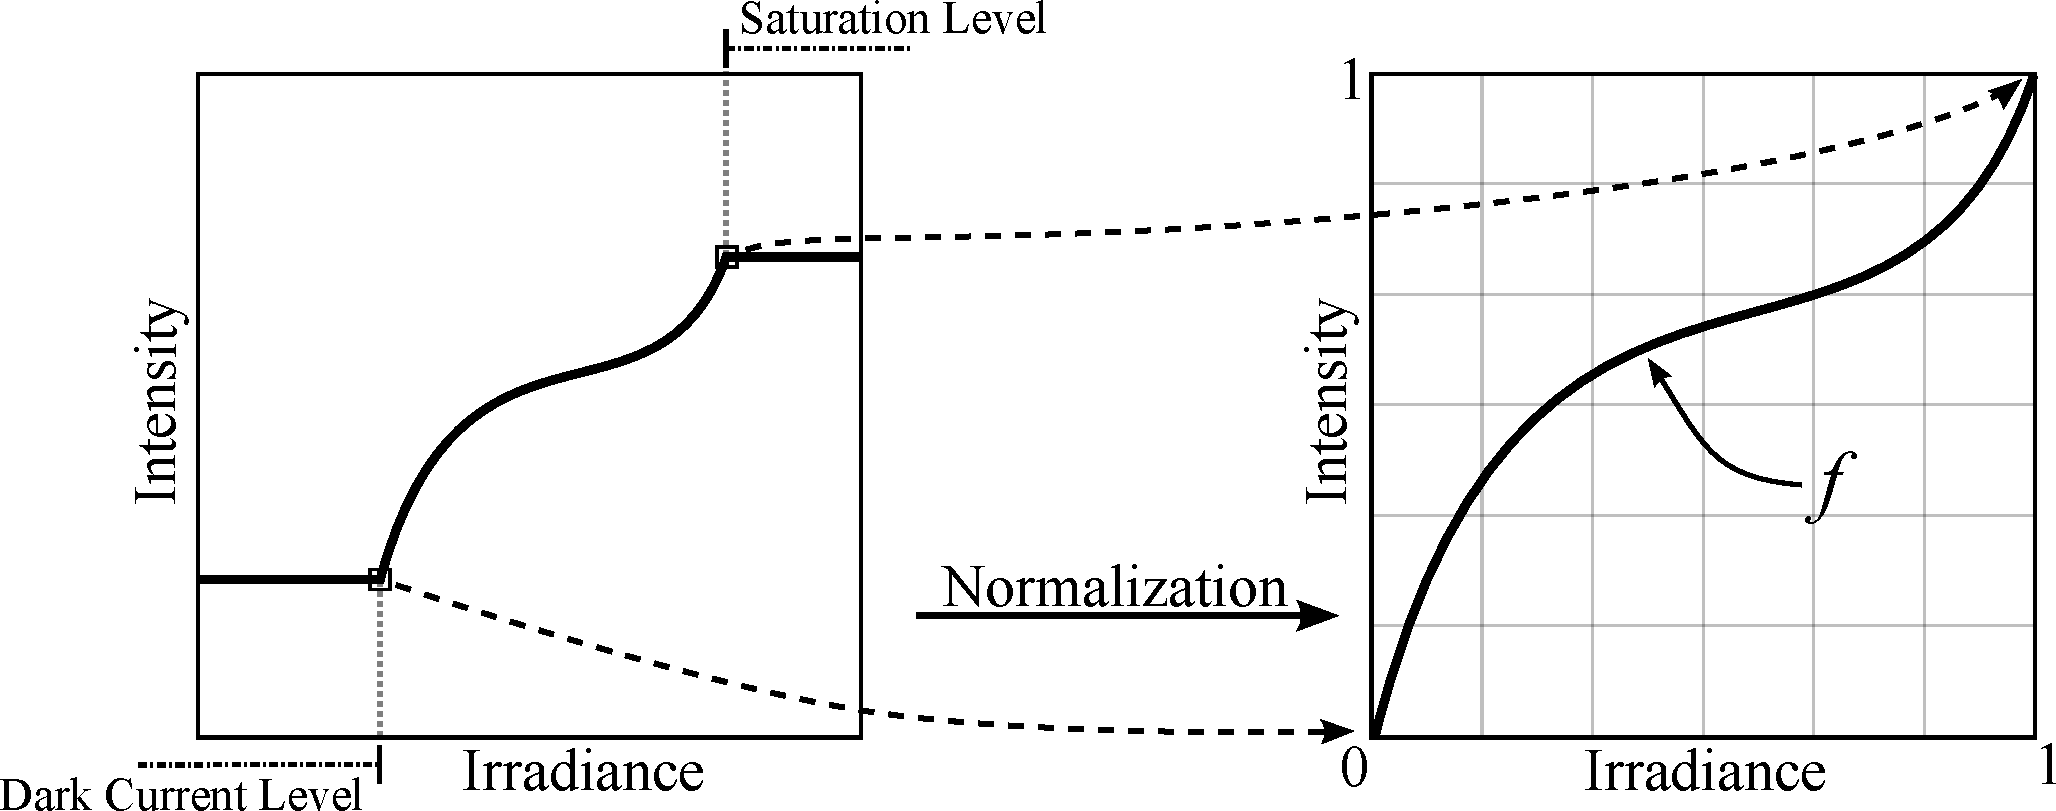
\includegraphics[width=0.8\linewidth]{images/crf_normalization.pdf}
	\caption[CRF normalization]{CRF normalization, inspired by M. Grossberg and S. Nayar. The left figure shows an example mapping from irradiance to intensity. The current levels (darkness and saturation) can not be recovered. Hence, they get cut off during the normalization process. The right figure shows the result of the normalization, a function which is called the camera response $f$. Both, domain and codomain lie within the range $[0; 1]$.}
	\label{fig:crfnormalization}
\end{figure}